\begin{figure}[H]
\centering
  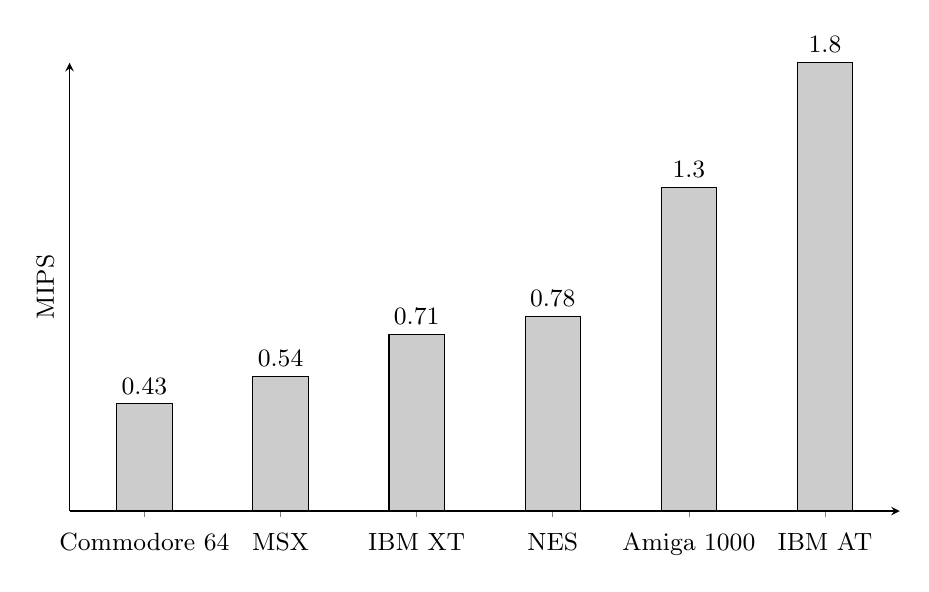
\begin{tikzpicture}[font=\small]
    \begin{axis}[
      width=\textwidth,
      height=0.6\textwidth,
      ybar=6pt,
      bar width=20pt,
      ylabel={MIPS},
      ymin=0,
      ytick=\empty,
      xtick=data,
      axis x line=bottom,
      axis y line=left,
      enlarge x limits=0.11,
      symbolic x coords={Commodore 64, MSX, IBM XT, NES, Amiga 1000, IBM AT},
      xticklabel style={anchor=base,yshift=-\baselineskip},
      nodes near coords={\pgfmathprintnumber\pgfplotspointmeta}
    ]
      \addplot[fill=black!20,draw=black] coordinates {
        (Commodore 64, 0.43)
        (MSX, 0.54)
        (IBM XT, 0.71)
        (NES, 0.78)
        (Amiga 1000,1.3)
        (IBM AT, 1.8)
      };
    \end{axis}
   \end{tikzpicture}
   \caption{Consoles\protect\footnotemark and IBM PC CPU comparison (MIPS)\protect\footnotemark $^,$\protect\footnotemark.}
   \label{fig:ems_xms_layout}
 \end{figure}
 \addtocounter{footnote}{-2}
 \footnotetext{The Commodore 64 uses a MOS 6510 CPU running at 1MHz. The MSX uses a Zilog Z80 running at 3.6MHz. The Amiga 1000 has a Motorola 68000 CPU  running at 7.16 MHz. The NES uses a Ricoh 2A03 CPU running at 1.8 MHz.}
 \stepcounter{footnote}
 \footnotetext{Million Instructions Per Second.}
 \stepcounter{footnote}
 \footnotetext{Gamicus Fandom: https://gamicus.fandom.com/wiki/Instructions\_per\_second.}
